\documentclass[a4paper, 12pt]{article}
    % General Document formatting
    \usepackage[margin=0.7in]{geometry}
    \usepackage[parfill]{parskip}
    \usepackage[utf8]{inputenc}
    \usepackage{graphicx}
    \usepackage{amsthm}
    \usepackage{amsmath}
    \usepackage{mathtools}

\newtheorem{mydef}{Definici\'on}
\newtheorem{mytheo}{Teorema}

\begin{document}
\title{Proyecto de Programaci\'on Declarativa}
\author{
   Adrian Gonz\'alez S\'anchez C412\\
   \texttt{https://github.com/adriangs1996}
   \and
   Eliane Puerta Cabrera C412\\
   \texttt{https://github.com/NaniPuerta}
}
\maketitle
\section*{Orientaci\'on}
\paragraph{}
En el Sudoku Hidato, el objetivo es rellenar el tablero con números consecutivos que se conectan
horizontal, vertical o diagonalmente. En cada juego de Hidato, los números mayor y menor
están marcados en el tablero. Todos los números consecutivos están adyacentes de forma vertical,
horizontal o diagonal. Hay algunos números más en el tablero para ayudar a dirigir al jugador
sobre cómo empezar a resolverlo y para asegurarse de que ese Hidato tiene solución única. Se
suele jugar en una cuadrícula como Sudoku pero también existen tableros hexagonales u otros más
irregulares con figuras como corazones, calaveras, etc. Cada puzzle de Hidato creado
correctamente debe tener solución única.

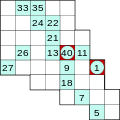
\includegraphics{HidatoExample.png}
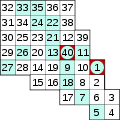
\includegraphics{HidatoExampleSolved.png}

\section*{Modelaci\'on}
\paragraph{}
Antes de atacar el problema de generar los tableros y resolverlos, es necesario tener un modelo computacional
del juego. Al ser un juego de tablero, y las restricciones que imponen el juego, lo m\'as adecuado consideramos
que sea un grafo donde los v\'ertices son las casillas del tablero. Cada v\'ertice representado por una coordenada
$(x,y)$ está conectado con su 8-vecindad, a excepci\'on, por supuesto, de las casillas de las esquinas y bordes. Adem\'as a cada
casilla del tablero debemos asignarle un label con un n\'umero $x\in[1, 2, ..., n]$ donde $n$ es el n\'umero de casillas disponibles
en el tablero. Estos labels vienen prefijados en las casillas que conocemos su valor. Dicho esto, el problema de resolver el Sudoku
Hidato se traduce en encontrar un camino Hamiltoniano en este grafo y asignar a cada v\'ertice sin label en este camino, un n\'umero de
forma que aparezcan de manera ordenada y creciente todos los valores $[1, 2, ..., n]$.

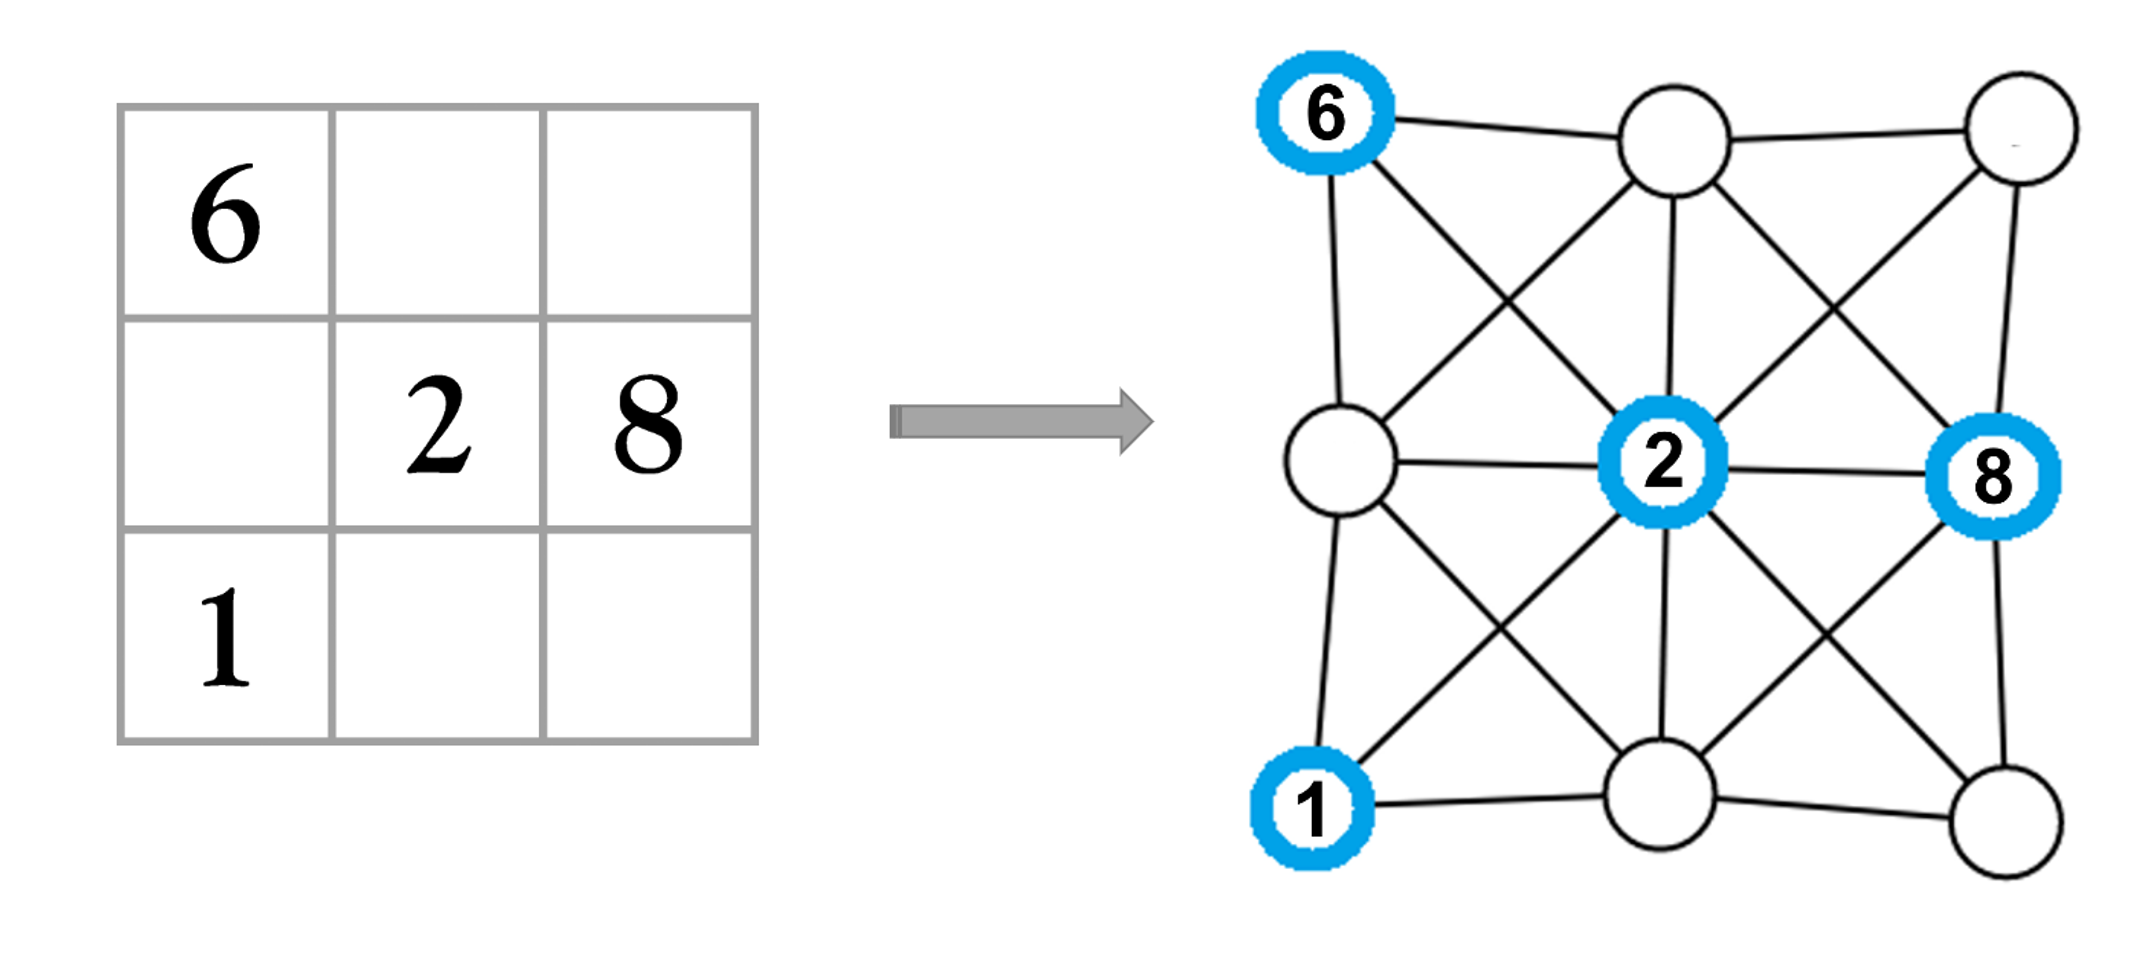
\includegraphics[scale=.2]{HidatoToGraph.png}
\paragraph{}
Desde el punto de vista program\'atico, definimos dos estructuras, una a utilizar en la soluci\'on del problema,
y la otra a utilizar en la generaci\'on. El punto de uni\'on de ambos algoritmos es el m\'etodo \textbf{boardToString}
el cual es utilizado por el generador para devolver un \textbf{[String]} que luego puede ser consumida por el m\'etodo
\textbf{makeBoard} que devuelve un \textbf{BoardProblem} que es la estructura usada para resolver el juego.

\section*{Resoluci\'on de un tablero}
\paragraph{}
En el archivo \textbf{src/Lib.hs} encontramos todas las definiciones necesarias para crear el m\'etodo
de resoluci\'on. Se define la estructura \textbf{BoardProblem} que engloba los datos necesarios sobre el
tablero:

\begin{enumerate}
   \item \textbf{cells}: Representa las celdas del tablero. Es un diccionario anidado de enteros de modo
         que podemos acceder a la casilla (x, y) de la siguiente forma: $dict[x][y]$.
   \item \textbf{onePos}: Posicion del 1 en el tablero.
   \item \textbf{endVal}: M\'aximo valor del tablero.
   \item \textbf{givens}: Valores prefijados del tablero. Estos valores son inicialmente insertados en \textbf{cells}.
\end{enumerate}

\paragraph{}
En este m\'odulo se presentan adem\'as varias funciones auxiliares que permiten insertar un valor en el tablero (\textbf{tupIns}),
obtener el valor de la casilla (x,y), imprimir en consola un tablero y parsear una lista de strings y convertirlas en un tablero.
Una funci\'on fundamental es \textbf{isSolved} la cual determina si un tablero ya est\'a resuelto comprobando si no existen celdas
vac\'ias y que se pueda llegar desde el 1 hasta \textbf{endVal} en un camino Hamiltoniano, incrementando el valor buscado en cada momento.

\paragraph{}
El coraz\'on de la resoluci\'on es la funci\'on \textbf{bruteForceHidato} que se encuentra en el m\'odulo
\textbf{src/Hidato.hs}. Esta funci\'on tiene la siguiente signatura:

\texttt{bruteForceHidato :: BoardProblem -> [IntMap (IntMap Int)]}

la cual devuelve una lista de tableros pues el algoritmo no requiere que los tableros tengan soluci\'on \'unica, es perfectamente
capaz de encontrar todas las soluciones del tablero que se le pase. Por supuesto, a la hora de engranar la aplicaci\'on, garantizamos
la generaci\'on de tableros \'unicos y un paso importante en este proceso es pedir soluciones a demanda, aprovechando el sistema lazy de evaluaci\'on
de Haskell, de este algoritmo sobre un tablero
espec\'ifico y si en algun momento obtenemos m\'as de una, sabemos que ese tablero no tiene soluci\'on \'unica y por tanto no es v\'alido.

La implementaci\'on de esta funci\'on es b\'asicamente un DFS empezando por las coordenadas del 1 (guardadas en \textbf{onePos}), o sea intentamos en cada
paso, que nos encontramos en un v\'ertice con label $l_i$, asignarle a alg\'un vecino de dicho v\'ertice que no tenga label, el label $l_{i+1}$ y luego
pasar a visitar ese vecino. Hay varios casos:

\begin{enumerate}
   \item El tablero est\'a resuelto, en dicho caso se devuelve.
   \item El v\'ertice que estamos visitando no tiene vecinos disponibles, en dicho caso se devuelve una lista vac\'ia (no es soluci\'on).
   \item El label que queremos colocar se encuentra en alguno de los vecinos del v\'ertice que estamos visitando, en dicho caso
         pasamos a visitar ese vecino e intentamos colocar el label $l_{i+1}$.
   \item Recursivamente insertamos el label que queremos colocar en alg\'un vecino disponible y pasamos a visitar cada uno de esos vecinos.
\end{enumerate}

El algoritmo solo explora las formas v\'alidas de colocar los labels, adem\'as intenta construir un camino v\'alido lo m\'as largo
posible, lo que en tableros con soluci\'on \'unica, lleva a encontrar la respuesta de una manera bastante r\'apida, permitiendo
resolver tableros decentemente grandes.

Los siguientes ejemplos fueron generados y resueltos en aproximadamente 0.00104s en una Dell Inspiron-7548 con 12GB de RAM y
un Intel COREi7 de n\'ucleo. Corresponden a tableros de 100 y 81 casillas respectivamente.

\begin{verbatim}
    $ ./SudokuHidato-exe -s
            30  0            
         35 33  0  0         
      38  0 34  0 27  0      
   40  0  0       25  0 22   
43  0  0             23  0 20
 0 45  0             17 18  0
   47 48  0       13 15  0   
       3  0  1 11  0  0      
          0  7  9  0         
             0  0            

            30 29            
         35 33 31 28         
      38 36 34 32 27 26      
   40 39 37       25 24 22   
43 42 41             23 21 20
44 45 46             17 18 19
   47 48  2       13 15 16   
       3  4  1 11 12 14      
          5  7  9 10         
             6  8       
\end{verbatim}

\begin{verbatim}
    $./SudokuHidato-exe -s
       0  0 29  0 26      
      33  0  0  0  0      
      36 35  0            
      38  0  0        0  2
44 43 41  0  0  0  0  0  1
 0  0  0  0  0 18 10  0  0
 0 48  0  0  0  0  0  0  0
50  0                 0  0
52 53                13  0

      32 31 29 28 26      
      33 34 30 25 27      
      36 35 24            
      38 37 23        3  2
44 43 41 39 22  9  8  4  1
45 46 42 40 21 18 10  7  5
49 48 47 20 19 17 16 11  6
50 51                15 12
52 53                13 14

\end{verbatim}

\section*{Generaci\'on}
\paragraph{}
La generaci\'on de tableros es quiz\'as la parte m\'as interesante del proyecto. Partamos primeramente de la
base de que necesitamos que cada tablero tenga una soluci\'on \'unica (de lo contrario, generar una matriz
y llenarla arbitrariamente garantizando que siempre exista soluci\'on es un trabajo trivial). La idea general
para generar los tableros se basa en:

\begin{enumerate}
   \item \textit{Generar una matriz de $N$x$M$ casillas.}
   \item \textit{"Tachar" algunas casillas para darle alguna forma al tablero.}
   \item \textit{Ubicar aleatoriamente el 1 y el m\'aximo valor del tablero.}
   \item \textit{Hallar un camino de Hamilton con las labels correctamentes colocados.}
   \item \textit{Eliminar algunos labels del tablero.}
   \item \textit{Comprobar que el tablero tiene soluci\'on \'unica.}
\end{enumerate}

\paragraph{}
La implementaci\'on de estos \textit{guidelines} se consolida en el m\'odulo \textbf{src/HidatoBoard.hs},
spec\'ificamente con la funci\'on:

\begin{verbatim}
   generateBoard :: Int -> [String]
\end{verbatim}

cuyo p\'arametro es un entero que utilizamos como semilla para generar los n\'umeros
aleatorios y su resultado es una lista de strings con el siguiente formato:

\begin{enumerate}
   \item Cada fila del tablero corresponde a un string de la lista.
   \item Cada casilla de la fila se separa en el string por un espacio.
   \item Los posibles elementos de cada casilla son :
         \begin{enumerate}
            \item ".": Indica que la casilla es inv\'alida (est\'a tachada, estas se muestran en consola como espacios en blanco).
            \item "0": Indica que esta casilla est\'a vac\'ia (Hay que ponerle su label).
            \item X: Donde X es cualquier entero.
         \end{enumerate}
\end{enumerate}

\textbf{generateBoard} primeramenta selecciona un tablero aleatoriamente de una lista de \textit{templates} definidas
previamente por nosotros:

\begin{verbatim}
   generateBoard randSeed = boardToStrings (makeHidatoBoard brd randSeed)
    where 
      brd = selectBoard (genRandInt randSeed)
\end{verbatim}

\paragraph{}
aunque pudi\'eramos realizar esta fase de una forma completamente aleatoria (este proceso corresponde a los tres primeros
pasos definidos en los \textit{guidelines}), seleccionar de un conjunto de templates nos permite crear tableros con formas
bien definidas (Cruces y rombos, por ejemplo), lo que hace un poco m\'as atractivos los tableros generados. Estos templates
no son m\'as que las dimensiones del tablero ($N$ y $M$) con la cual se genera una matriz completamente vac\'ia (todos los valores
en 0), y una lista de pares $(x,y)$ representando un conjunto de posiciones tal que, el tablero en la posicion $(x, y)$ est\'a tachado.

\paragraph{}
Con el tablero vac\'io en mano, pasamos al pr\'oximo paso del algoritmo: Generar un camino Hamiltoniano con los labels correctamente
colocados, de lo cual se ocupa \textbf{makeHidatoBoard}.

\paragraph{}
Espera un segundo..., ese problema es el mismo que el de resolver el Hidato !?. La verdad es que no, en este caso, solo
necesitamos encontrar \textit{un} camino Hamiltoniano a partir de una posici\'on original, luego los labels los podemos colocar
en orden ascendente y tenemos nuestra respuesta.

\paragraph{}
Espera de nuevo..., encontrar un camino Hamiltoniano es NP-Hard verdad !?. True, pero en este caso, este grafo es basado en una
matriz, conecatdo en 8-vecindades (como un tablero de Ajedrez ;) ), y el problema de recorrer este tablero en un camino Hamiltoniano es conocido como \textbf{Knight's Tour},
el cual se soluciona en tiempo $O(n)$ con la heur\'istica de \textbf{Warnsdorff}. Esta heur\'istica es un caso t\'ipico de \textit{greedy}
en el cual el tablero se divide en cuadrículas m\'as chicas de acuerdo a la cantidad de movimientos disponibles del caballo (en el caso
del Knight's Tour Problem) y en cada momento, se mueve hacia la casilla que permite la menor cantidad de movimientos
posibles y que no haya sido visitada. Para poder aplicarlo en nuestro problema, debemos generalizar esta heur\'istica, y una generalizaci\'on inmediata es siempre
moverse al v\'ertice de menor \textit{degree}. Esta es b\'asicamente la idea detr\'as de la funci\'on:

\begin{verbatim}
   buildTreeWarnsdorff
    :: PathTree Int
    -> Board
    -> Coordinates
    -> Int
    -> Int
    -> Int
    -> (Int, PathTree Int)
\end{verbatim}

la cual toma los m\'odulos \textbf{src/BoatdGen.hs, src/PathTree.hs, src/MyMatrix.hs, src/Solve.hs} para
poder calcularse (junto con otras funcionalidades inherentes a las estructuras definidas para hacer m\'as
c\'omoda la implementaci\'on).

Una vez que rellenamos el tablero con el camino Hamiltoniano, pasamos a los \'ultimos dos pasos de los \textit{guidelines},
o sea, vaciar algunas casillas, y garantizar que la soluci\'on sea \'unica. Para lograr esto, la funci\'on

\begin{verbatim}
   getUniqueBoard :: (Eq a) => Board -> PathTree a -> Int -> Board
\end{verbatim}
selecciona aleatoriamente una coordenada de la lista de elementos incorporados al tablero (en esta lista, no aparecen
las coordenadas del 1 ni del m\'aximo valor del tablero), la elimina y luego corre el m\'etodo \textbf{bruteForceHidato}, del
cual intenta extraer 2 soluciones, aprovech\'andose del sistema lazy de evaluaci\'on de Haskell, si la cantidad de soluciones
es 1, entonces es seguro vaciar esa casilla, de lo contrario, el valor de esa casilla se restaura, y esa coordenada se elimina
de la lista de coordenadas. Este proceso se ejecuta mientras la lista de coordenadas no quede vac\'ia.

\paragraph{}
Una vez que tenemos nuestro tablero generado, se le pasa a la funci\'on

\begin{verbatim}
   boardToStrings :: Board -> [String]
\end{verbatim}
que devuelve la lista de strings necesarias para luego poderse parsear, y ser utilizada por el solver.

\section*{Implementaci\'on de la app}
El m\'odulo \textbf{app/Main.hs} se ocupa de engranar los algorimos implementados en una simple interfaz
de usuario basada en l\'ineas de comando para correr tanto el generador, como el solver. Para implementar
esta funcionalidad, hicimos uso extensivo del \textbf{IO Monad} junto con el m\'odulo \textbf{GetOpt}

\begin{verbatim}
   import           System.Console.GetOpt
\end{verbatim}
donde usamos principalmente la funci\'on \textbf{getOpt} para parsear los argumentos devueltos por 
\textbf{getArgs} y agruparlos en flags, de acuerdo las opciones definidas en \textit{options}, de la 
siguiente forma:

\begin{verbatim}
   parse :: [String] -> IO [Flag]
parse argv = case getOpt Permute options argv of
    (args, _, []) -> do
        if Help `elem` args
            then do
                hPutStrLn stderr (usageInfo header options)
                exitWith ExitSuccess
            else return (nub args)

    (_, _, err) -> do
        hPutStrLn stderr (concat err ++ usageInfo header options)
        exitWith $ ExitFailure 1
    where header = "Usage: SudokuHidato [-rsftg]"
\end{verbatim}

\section*{Compilar el proyecto y usar la app}
\paragraph{}
El proyecto usa el sistema de compilado para Haskell \textbf{stack}. Obtener un compilado debe ser tan f\'acil como ejecutar los siguientes
comandos:

\begin{verbatim}
    $ stack setup
    $ stack build
\end{verbatim}

Adem\'as proveemos un compilado SudokuHidato-exe (\textbf{Linux}), que se puede utilizar en caso de que no se quiera compilar el proyecto.
Esta app es un programa de l\'inea de comandos que ofrece las siguientes opciones:

\begin{verbatim}
  $ ./SudokuHidato-exe --help
  Usage: SudokuHidato [-rsftg]
            --help                Print this help message
  -g COUNT  --generate=COUNT      Generate COUNT boards and shows them
  -s        --genandsolve         Generate 1 board, prints it, solves it and 
                                  prints the solution
  -t FILE   --gentestfile=FILE    Generate 10 boards and save them in FILE
  -f FILE   --solvefromfile=FILE  Read boards in file and solve them
  -r FILE   --showFile=FILE       Read boards in file and show them
\end{verbatim}

Con el flag \textbf{-g} podemos generar una cantidad arbitraria de tableros y los imprime en consola
para resolverlos a mano o algo por el estilo. La generacion de tableros ocurre cada 1 segundo, pues
el tiempo actual se usa como semilla para la generaci\'on de numeros aleatorios. Por ejemplo:

\begin{verbatim}




    $ ./SudokuHidato-exe -g 3
       0 10  8  0  0      
       0 12  0  0  5      
      15 14  0            
       0 17  0        0 43
 0  0  0  0  0  1  0 45  0
23  0 32  0  0 38  0  0 47
 0 30  0 34 36  0  0 48  0
26  0                53  0
 0 28                 0 52


            47 48            
          0  0  0 44         
       0 39  0 42  0  0      
    0 36 38        0  5  1   
 0  0 34              0  0  0
 0 31 32             11  0  3
    0  0  0        0 12  0   
      26  0 22  0 15 13      
         23  0 18 16         
             0 19            


       0 24 26  0  0      
       0  0  0  0 30      
       0  0  0            
       0 34  0        0  0
 7  0  0  0 36  0  0 43 42
 0  9  0 15  0 38 46  0  0
 0  0  0 12  0  0  0 48  0
 0  4                 0 52
 1  2                53  0
\end{verbatim}

Con el flag \textbf{-s} se genera un tablero, se muestra y se soluciona. Por ejemplo

\begin{verbatim}
    $./SudokuHidato-exe -s

        0            
     0  0  0         
    0 18 15 12  0      
     0  0  0  1  0  0
           0  0  2   

       10            
    16 11  9         
    17 18 15 12  8      
    14 13  7  1  4  3
           6  5  2     
\end{verbatim}
Las otras tres opciones sirven para generar tableros y guardarlos para luego utilizarlos como
entrada para el algoritmo solucionador. Por ejemplo, con el flag \textbf{-t} generamos 10 tableros
y los guardamos en un archivo que se pasa como entrada en la l\'inea de comandos. Este archivo luego
puede ser mostrado o resuelto usando los flags \textbf{-f } o \textbf{-r}: Por ejemplo:

\begin{verbatim}
    $ ./SudokuHidato-exe -t test.txt
    $ ./SudokuHidato-exe -r test.txt
                 0 19            
             23 21  0 16         
           0 24  0  0 15  0      
       28 27 25       14 12  0   
    31  0  0             10  9  0
     0 33  0              0  0  5
       35  0  0        1  3  0   
          37  0 41  0  0  0      
             40 48 47  0         
                 0  0            

           0
     4  0  1
     6  0   

           0            
        0 10 12         
     6  0 11  0 14      
        0  0  3  0 17 18
              0  1  0   

        ......... omitidos los otros 7 por brevedad .........
\end{verbatim}
\begin{verbatim}
    $ ./SudokuHidato-exe -f test.txt
                20 19            
             23 21 18 16         
          26 24 22 17 15 13      
       28 27 25       14 12 11   
    31 30 29             10  9  6
    32 33 34              8  7  5
       35 36 38        1  3  4   
          37 39 41 42 43  2      
             40 48 47 44         
                46 45            

           2
     4  3  1
     6  5   

           9            
        8 10 12         
     6  7 11 13 14      
        5  4  3 15 17 18
              2  1 16
    ............... omitidos los otros 7 por brevedad ............
\end{verbatim}

Por supuesto, si se quieren utilizar m\'as casos de prueba en un archivo, se puede
hacer uso de los poderes de \textbf{bash}.
\end{document}
